%\documentclass[tikz,14pt,border=10pt]{standalone}
\documentclass{article}
\usepackage[utf8]{inputenc}
\usepackage{amsmath}
\usepackage{amsfonts}              	% for blackboard bold, etc
\usepackage{amsthm}                	% better theorem
\usepackage{amssymb}
\usepackage{mathtools}
\usepackage{graphicx}
\usepackage{epstopdf}
\renewcommand{\baselinestretch}{1.5} 


\usepackage[all]{xy}
%\usepackage{textcomp}
%\usetikzlibrary{shapes,arrows}
\usepackage{tikz}
\usepackage{pgfplots} 
\usetikzlibrary{shapes,arrows,positioning,calc}

\tikzset{
block/.style = {draw, fill=white, rectangle, minimum height=3em, minimum width=3em},
tmp/.style  = {coordinate}, 
sum/.style= {draw, fill=white, circle, node distance=1cm},
input/.style = {coordinate},
output/.style= {coordinate},
pinstyle/.style = {pin edge={to-,thin,black}
}
}

\title{ECE355 - Homework IV}
\author{Dantas de Lima Melo, Vinícius \\ \small{1001879880}}
\date{September 2014}

\begin{document}

\maketitle

\setcounter{section}{1}
\section{}
    \setcounter{subsection}{21}
    \subsection{} For each of the following pairs of waveforms, use the convolution integral to find the response $y(t)$ and sketch the results.
    \begin{enumerate}
        \item[(a)]
            \begin{equation*}
                \left\{\begin{array}{ccl}
                    x(t)&=& e^{-\alpha t}u(t)  \\
                    h(t)&=& e^{-\beta t}u(t)
                \end{array}\right.
            \end{equation*}
            Use both cases: $\alpha = \beta$, and $\alpha \neq \beta$. \\
            \begin{equation} \label{eq:1.27a1}
                \begin{array}{l}
                 y(t) = x(t)*h(t) = \int_{-\infty}^{+\infty} e^{-\alpha \tau}u(\tau)e^{-\beta (t-\tau)}u(t-\tau) d\tau  \\
                 \Rightarrow y(t) = e^{-\beta t} \int_{-\infty}^{+\infty} e^{-\alpha \tau}u(\tau)e^{\beta \tau}u(t-\tau) d\tau \\
                 \Rightarrow y(t) = e^{-\beta t} \int_{0}^{+\infty} e^{-\alpha \tau}e^{\beta \tau}u(t-\tau) d\tau \\ 
                \Rightarrow y(t) = e^{-\beta t} \int_{0}^{t} e^{-\alpha \tau}e^{\beta \tau} d\tau = e^{-\beta t} \int_{0}^{t} e^{\tau(\beta-\alpha)} d\tau\\ 
                \end{array}
            \end{equation}
            From (\ref{eq:1.27a1}), taking $\alpha = \beta$, we have: \\
            \begin{equation*}
            y(t) = e^{-\beta t} \int_{0}^{t} e^{\tau(\beta-\alpha)} d\tau = e^{-\beta t} \int_{0}^{t} d\tau = te^{-\beta t}u(t)
            \end{equation*}
            We multiply $y(t)$ by $u(t)$ because this signal only exists for $t>0$, since $x(t)$ and $h(t)$ only exist for $t>0$.
            Now, going back to (\ref{eq:1.27a1}), and taking $\alpha \neq \beta$:
            \begin{equation*}
            y(t) = e^{-\beta t} \int_{0}^{t} e^{\tau(\beta-\alpha)} d\tau = e^{-\beta t} \frac{e^{\tau(\beta-\alpha)}}{\beta-\alpha}\biggl|_{\tau=0}^{t} = e^{-\beta t} \frac{e^{t(\beta-\alpha)}}{\beta-\alpha} = e^{-\beta t}\left( \frac{e^{t(\beta-\alpha)}-1}{\beta-\alpha}\right)u(t)
            \end{equation*}
            \begin{equation*}
            \therefore y(t) = \left\{\begin{array}{lr}
            te^{-\beta t}u(t) & \textrm{, if } \alpha=\beta\\
            e^{-\beta t}\left( \frac{e^{t(\beta-\alpha)}-1}{\beta-\alpha}\right)u(t) & \textrm{, if } \alpha \neq \beta
            \end{array}\right.
            \end{equation*}
            \begin{minipage}{0.5\textwidth}
            \centering $\alpha=\beta$ \\
            \includegraphics[width=2.65in]{Images/graph1.eps}
            \end{minipage}
            \begin{minipage}{0.5\textwidth}
            \centering $\alpha\neq\beta$ \\
            \includegraphics[width=2.65in]{Images/graph2.eps}
            \end{minipage}
            
        \item[(b)]
            \begin{equation*} 
                \left\{\begin{array}{ccl}
                    x(t)&=& u(t)-2u(t-2)+u(t-5)  \\
                    h(t)&=& e^{2t}u(1-t)
                \end{array}\right.
            \end{equation*}
            So we can calculate $y(t)$:
            \begin{equation*}
                \begin{array}{l}
                    y(t) = x(t)*h(t) = \int_{-\infty}^{+\infty} [u(\tau)-2u(\tau-2)+u(\tau-5)]e^{2(t-\tau)}u(1-t+\tau) d\tau  \\
                    \Rightarrow y(t) = \int_{t-1}^{+\infty} [u(\tau)-2u(\tau-2)+u(\tau-5)]e^{2(t-\tau)} d\tau \\
                    \Rightarrow y(t) = \int_{t-1}^{+\infty} e^{2(t-\tau)}u(\tau)d\tau -2\int_{t-1}^{+\infty} e^{2(t-\tau)}u(\tau-2)d\tau+\int_{t-1}^{+\infty}e^{2(t-\tau)}u(\tau-5) d\tau \\
                    \Rightarrow y(t) = e^{2t}[\int_{t-1}^{+\infty} e^{-2\tau}u(\tau)d\tau -2\int_{t-1}^{+\infty} e^{-2\tau}u(\tau-2)d\tau+\int_{t-1}^{+\infty}e^{-2\tau}u(\tau-5) d\tau] \\
                \end{array}
            \end{equation*}
            Now we need to break it into different cases (pieces). \\
            For $\tau < 0 \Leftrightarrow t < 1$:
            \begin{equation} \label{eq:1.27b1}
                \begin{array}{l}
                    y(t) =  e^{2t}[\int_{t-1}^{+\infty} e^{-2\tau}u(\tau)d\tau -2\int_{t-1}^{+\infty} e^{-2\tau}u(\tau-2)d\tau+\int_{t-1}^{+\infty}e^{-2\tau}u(\tau-5) d\tau] \\
                    \Rightarrow y(t) =  e^{2t}[\int_{0}^{+\infty} e^{-2\tau}d\tau -2\int_{2}^{+\infty} e^{-2\tau}d\tau+\int_{5}^{+\infty}e^{-2\tau} d\tau] \\
                    \Rightarrow y(t) =  e^{2t}[\int_{0}^{2} e^{-2\tau}d\tau + \int_{2}^{+\infty} e^{-2\tau}d\tau -\int_{2}^{+\infty} e^{-2\tau}d\tau - \int_{2}^{+\infty} e^{-2\tau}d\tau+\int_{5}^{+\infty}e^{-2\tau} d\tau] \\
                    \Rightarrow y(t) =  e^{2t}[\int_{0}^{2} e^{-2\tau}d\tau - \int_{2}^{5} e^{-2\tau}d\tau - \int_{5}^{+\infty} e^{-2\tau}d\tau+\int_{5}^{+\infty}e^{-2\tau} d\tau] \\
                    \Rightarrow y(t) =  e^{2t}[\int_{0}^{2} e^{-2\tau}d\tau - \int_{2}^{5} e^{-2\tau}d\tau] = e^{2t}\left[\frac{e^{-2\tau}}{-2}\biggl|_{\tau=0}^{2} - \frac{e^{-2\tau}}{-2}\biggl|_{\tau=2}^{5} \right] \\
                    \Rightarrow y(t) = \frac{e^{2t}}{2}[1-2e^{-4}+e^{-10}]
                  
                \end{array}
            \end{equation} 
            For $1 < t < 3$:
            \begin{equation} \label{eq:1.27b2}
                \begin{array}{l}
                   y(t) =  e^{2t}[\int_{t-1}^{+\infty} e^{-2\tau}u(\tau)d\tau -2\int_{t-1}^{+\infty} e^{-2\tau}u(\tau-2)d\tau+\int_{t-1}^{+\infty}e^{-2\tau}u(\tau-5) d\tau] \\
                   \Rightarrow y(t) =  e^{2t}[\int_{t-1}^{+\infty} e^{-2\tau}d\tau -2\int_{2}^{+\infty} e^{-2\tau}d\tau + \int_{5}^{+\infty} e^{-2\tau}d\tau] \\
                   \Rightarrow y(t) = e^{2t}[\int_{t-1}^{2} e^{-2\tau}d\tau + \int_{2}^{+\infty} e^{-2\tau}d\tau -2\int_{2}^{+\infty} e^{-2\tau}d\tau + \int_{5}^{+\infty} e^{-2\tau}d\tau] \\
                   \Rightarrow y(t) = e^{2t}[\int_{t-1}^{2} e^{-2\tau}d\tau -\int_{2}^{5} e^{-2\tau}d\tau -\int_{5}^{+\infty} e^{-2\tau}d\tau + \int_{5}^{+\infty} e^{-2\tau}d\tau] \\
                   \Rightarrow y(t) = e^{2t}[\int_{t-1}^{2} e^{-2\tau}d\tau -\int_{2}^{5} e^{-2\tau}d\tau] \\
                   \Rightarrow y(t) = \frac{e^{2t}}{2}[e^{2(1-t)}-2e^{-4}+e^{-10}]
                \end{array}
            \end{equation}
            For $3 < t < 6$:
            \begin{equation} \label{eq:1.27b3}
                \begin{array}{l}
                    y(t) =  e^{2t}[\int_{t-1}^{+\infty} e^{-2\tau}u(\tau)d\tau -2\int_{t-1}^{+\infty} e^{-2\tau}u(\tau-2)d\tau+\int_{t-1}^{+\infty}e^{-2\tau}u(\tau-5) d\tau] \\
                    \Rightarrow y(t) =  e^{2t}[\int_{t-1}^{+\infty} e^{-2\tau}d\tau -2\int_{t-1}^{+\infty} e^{-2\tau}d\tau+\int_{5}^{+\infty}e^{-2\tau} d\tau] \\
                    \Rightarrow y(t) = e^{2t}[-\int_{t-1}^{+\infty} e^{-2\tau}d\tau+\int_{5}^{+\infty}e^{-2\tau} d\tau] \\ 
                    \Rightarrow y(t) = e^{2t}[-\int_{t-1}^{5} e^{-2\tau}d\tau -\int_{5}^{+\infty} e^{-2\tau}d\tau +\int_{5}^{+\infty}e^{-2\tau} d\tau] = e^{2t}(\int_{t-1}^{5} -e^{-2\tau}d\tau) \\
                    \Rightarrow y(t) = \frac{e^{2t}}{2}e^{-2\tau}\biggl|_{\tau=t-1}^{5} = \frac{e^{2t}}{2}[e^{-10}-e^{2(1-t)}]
                \end{array}
            \end{equation}
            For $t > 6$:
            \begin{equation} \label{eq:1.27b4}
                \begin{array}{l}
                   y(t) =  e^{2t}[\int_{t-1}^{+\infty} e^{-2\tau}u(\tau)d\tau -2\int_{t-1}^{+\infty} e^{-2\tau}u(\tau-2)d\tau+\int_{t-1}^{+\infty}e^{-2\tau}u(\tau-5) d\tau] \\
                   y(t) = e^{2t}[\int_{t-1}^{+\infty} e^{-2\tau}d\tau -2\int_{t-1}^{+\infty} e^{-2\tau}d\tau+\int_{t-1}^{+\infty}e^{-2\tau} d\tau] = 0
                  
                \end{array}
            \end{equation}
            Putting (\ref{eq:1.27b1}), (\ref{eq:1.27b2}), (\ref{eq:1.27b3}) and (\ref{eq:1.27b4}) together: 
            \begin{equation*}
                y(t) = \left\{ \begin{array}{ll}
                 \frac{e^{2t}}{2}[1-2e^{-4}+e^{-10}] &\textrm{, if } t < 1  \\
                 \frac{e^{2t}}{2}[e^{2(1-t)}-2e^{-4}+e^{-10}]&\textrm{, if } 1 < t < 3 \\
                 \frac{e^{2t}}{2}[e^{-10}-e^{2(1-t)}]&\textrm{, if } 3 < t < 6 \\
                 0&\textrm{, if } t > 6
                \end{array}\right.
            \end{equation*}
            \begin{center}
                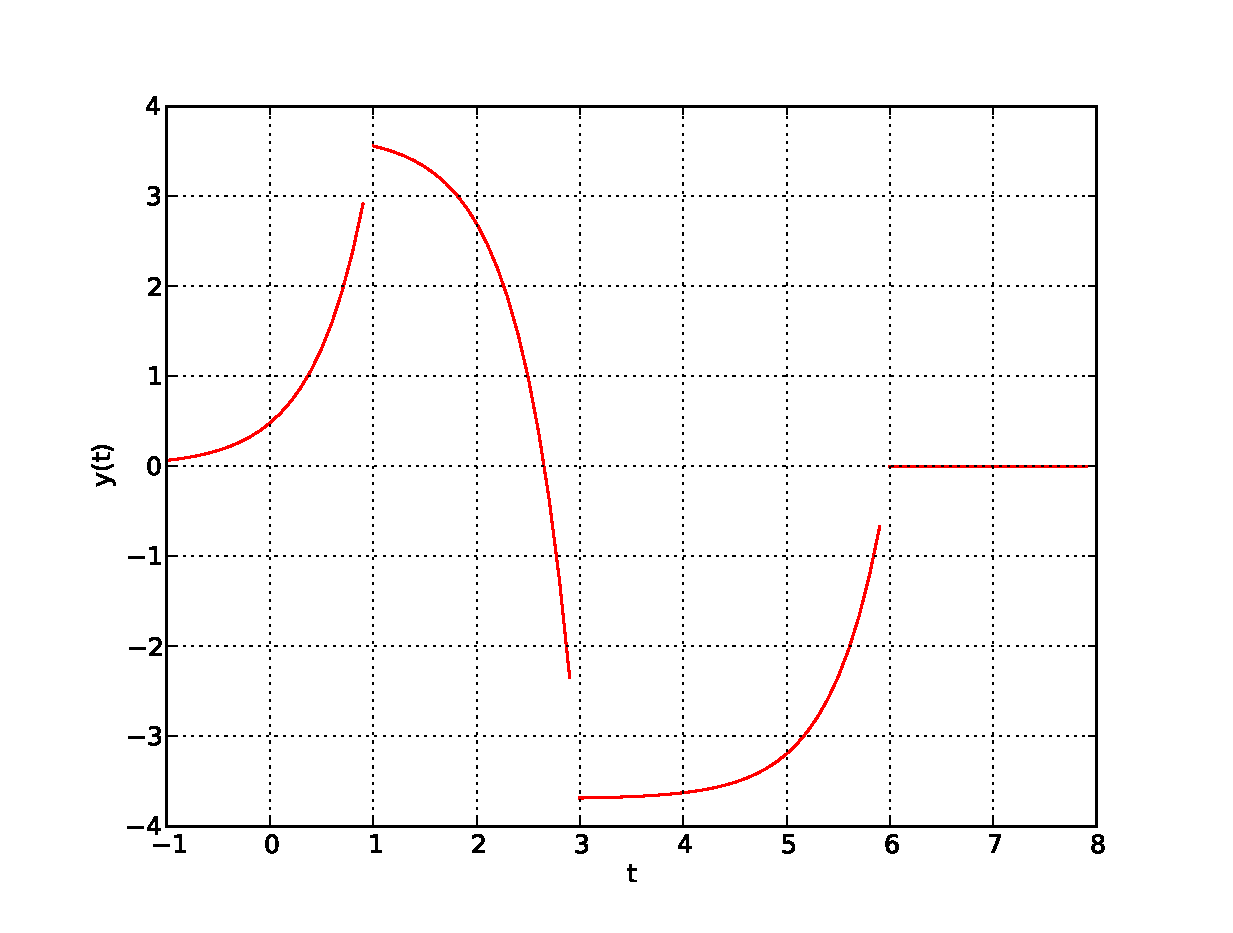
\includegraphics[width=2.65in]{Images/graph3.eps}
            \end{center}
        \item[(c)] 
             \begin{equation*}
                \left\{\begin{array}{ccl}
                    x(t)&=& sin(\pi t)[u(t)-u(t-2)]  \\
                    h(t)&=& 2[u(t-1)-u(t-3)]
                \end{array}\right.
            \end{equation*}
            So we can calculate $y(t)$:
            \begin{equation*}
                \begin{array}{l}
                    y(t) = x(t)*h(t) = \int_{-\infty}^{+\infty} sin(\pi \tau)[u(\tau)-u(\tau-2)]\cdot 2 \cdot [u(t-\tau-1)-u(t-\tau-3)] d\tau  \\
                \end{array}
            \end{equation*}
            From $[u(t-\tau-1)-u(t-\tau-3)]$, we have that $t-3 < \tau < t-1$. In addition, from $[u(\tau)-u(\tau-2)]$, we have that $0 < \tau < 2$. So:
            \begin{equation*} 
                \begin{array}{l}
                    y(t) =  2\int_{t-3}^{t-1} sin(\pi \tau) d\tau
                \end{array}
            \end{equation*}
            If $t < 1$, we will have the upper limit of integration less then $0$, but $\tau$ must be in the interval $(0,2)$, so $y(t) = 0$. In a similar way, if $t > 5$, $y(t) = 0$ because the lower limit would be greater then $2$. \\
            There are two possible situations remaining. The first situation is if $t - 3 < 0$, i.e., $t \in (1,3)$, the other one is if $t - 3 > 0$, i.e., $t \in (3,5)$. \\
            For the first case:
            \begin{equation} \label{eq:1.27b1}
                \begin{array}{l}
                    y(t) =  2\int_{0}^{t-1} sin(\pi \tau) d\tau = -2\frac{cos(\pi\tau)}{\pi} \biggl|_{\tau=0}^{t-1} = -\frac{2}{\pi} [cos(\pi(t-1)) - 1]\\
                    \Rightarrow y(t) = \frac{2}{\pi} [1 - cos(\pi(t-1))]
                \end{array}
            \end{equation}
            For the second case:
            \begin{equation} \label{eq:1.27b2}
                \begin{array}{l}
                    y(t) =  2\int_{t-3}^{2} sin(\pi \tau) d\tau = -2\frac{cos(\pi\tau)}{\pi} \biggl|_{\tau=t-3}^{2} = -\frac{2}{\pi} [1 - cos(\pi(t-3))]  \\
                    y(t) = \frac{2}{\pi} [cos(\pi(t-3))-1]
                \end{array}
            \end{equation}
            Putting \ref{eq:1.27b1} and \ref{eq:1.27b2} together with the previous results:
            \begin{equation*}
                y(t) = \left\{ \begin{array}{ll}
                 0 &\textrm{, if } t < 1  \\
                 \frac{2}{\pi} [1 - cos(\pi(t-1))]&\textrm{, if } 1 < t < 3 \\
                 \frac{2}{\pi} [cos(\pi(t-3))-1]&\textrm{, if } 3 < t < 5 \\
                 0&\textrm{, if } t > 5
                \end{array}\right.
            \end{equation*}
             \begin{center}
                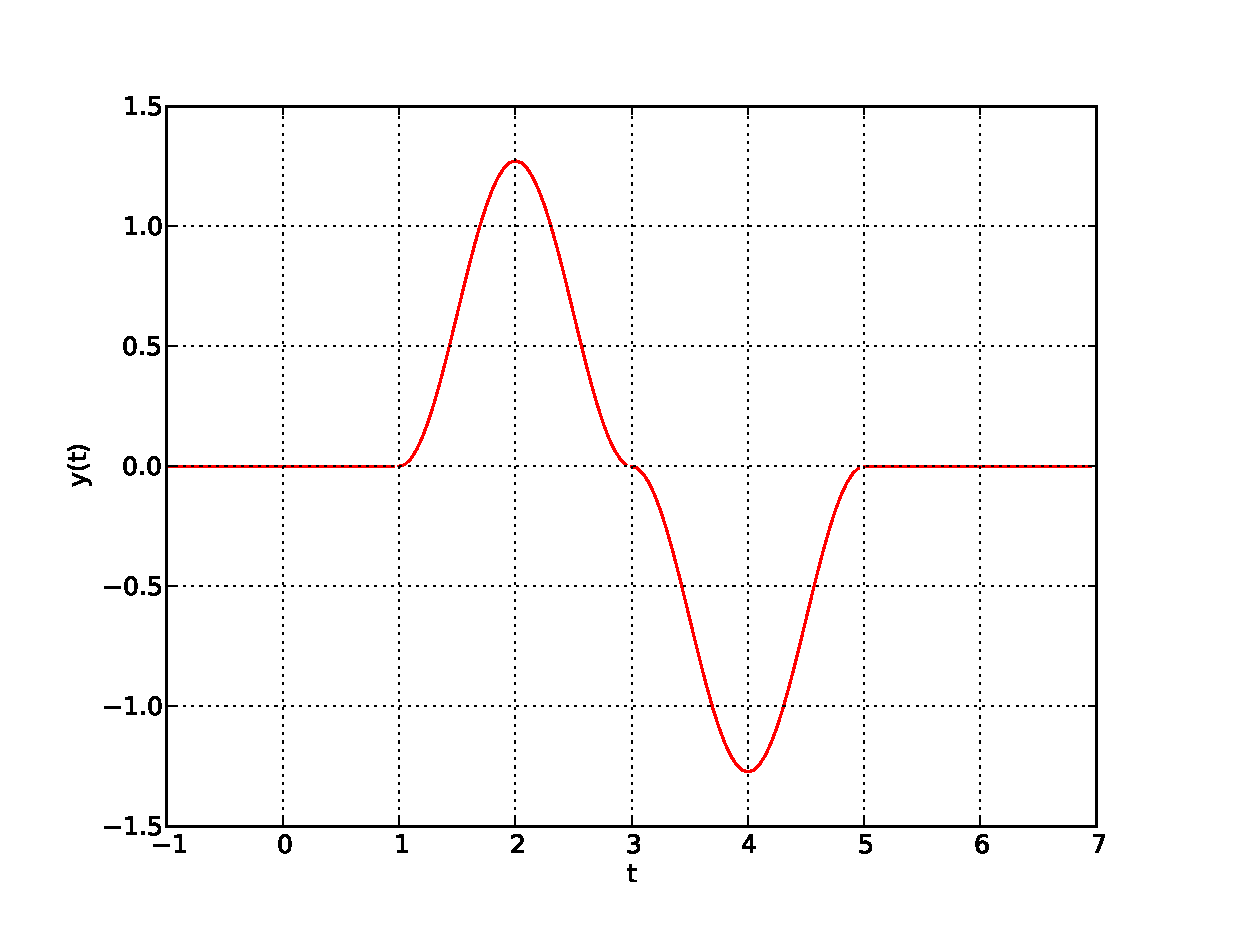
\includegraphics[width=2.65in]{Images/graph4.eps}
            \end{center}
    \end{enumerate}
    \setcounter{subsection}{28}
    \subsection{} Given $h(t)$, determinate if the system is either causal or stable.
        \begin{enumerate}
            \item[(a)] 
            \begin{equation*}
                h(t) = e^{-4t}u(t-2)
            \end{equation*}
            The system is causal because $h(t) = 0$ $\forall t < 0$. In addition, the system is stable as well because $\int_{-\infty}^{+\infty} |h(t)| dt = \frac{e^{-8}}{4} < +\infty$.
            \item[(b)]
            \begin{equation*}
                h(t) = e^{-6t}u(3-t)
            \end{equation*}
            The system is not causal because $h(t) \neq 0$ for some values of $t < 0$. In addition, the system is not stable because $\int_{-\infty}^{+\infty} |h(t)| dt = -\frac{e^{-6t}}{4}\biggl|_{-\infty}^{3} = +\infty$.
            \item[(c)]
            \begin{equation*}
                h(t) = e^{-2t}u(t+50)
            \end{equation*}
            The system is not causal because $h(t) \neq 0$ for some values of $t < 0$. However, the system is stable because $\int_{-\infty}^{+\infty} |h(t)| dt = -\frac{e^{-2t}}{4}\biggl|_{-50}^{+\infty} = \frac{e^{100}}{2} < +\infty$.
            \item[(d)]
            \begin{equation*}
                h(t) = e^{2t}u(-1-t)
            \end{equation*}
            The system is not causal because $h(t) \neq 0$ for some values of $t < 0$. However, the system is stable because $\int_{-\infty}^{+\infty} |h(t)| dt = -\frac{e^{2t}}{2}\biggl|_{-\infty}^{-1} = \frac{e^{-2}}{2} < +\infty$.
        \end{enumerate}
    \setcounter{subsection}{37}
    \subsection{} Draw a block diagram representation for the following systems
    \begin{enumerate}
        \item[(a)] $y[n] = \frac{1}{3}y[n-1]+\frac{1}{2}x[n]$\\
            \begin{tikzpicture}[auto, node distance=2cm,>=latex']

                \node [input, name=input] {};
                \node [input, below of=input] (constant1) {$\frac{1}{2}$};
                \node [input, below of=constant1] (constant2) {$\frac{1}{2}$};
                \node [sum, right of=input] (product1) {$\times$};
                \node [sum, right of=product1] (sum) {$+$};
                \node [input, below of=product1] (inv1) {};
                \node [input, below of=inv1] (inv2) {};
                \node [sum, right of=inv2] (product2) {$\times$};
                \node [input, below of=sum] (constant3) {$\frac{1}{3}$};
                \node [input, right of=sum] (inv3) {};
                %\node [block, right of=sum] (controller) {Controller};
                \node [block, right of=product2] (delay) {Delay};
                %\node [block, right of=sum, pin={[pinstyle]below:D},
                %        node distance=3cm] (delay) {Delay};

                %\draw [->] (controller) -- node[name=u] {$u$} (system);
                \node [output, right of=inv3] (output) {};
                %\node [block, below of=u] (measurements) {Measurements};
                %\coordinate [below of=sum] (measurements) {};
                \draw [draw,->] (input) -- node {$x[n]$} (product1);
                \draw [draw,->] (product1) --  (sum);
                \draw [draw,-] (constant1) -- node {$\frac{1}{2}$} (inv1);
                \draw [draw,->] (inv1) --  (product1);
                \draw [draw,-] (constant2) -- node {$\frac{1}{3}$} (inv2);
                \draw [draw,->] (inv2) --  (product2);
                \draw [draw,->] (product2) --  (sum);
                \draw [draw,->] (delay) --  (product2);
                \draw [-] (sum) -- (inv3);
                \draw [->] (inv3) -- (delay);
                \draw [->] (inv3) -- node [name=y] {$y[n]$}(output);
                %\draw [->] (y) |- (measurements);
                %\draw [-] (y) -- (constant2);
                %\draw [->] (measurements) -| node[pos=0.99] {$-$} 
                %\draw [->] (measurements) -| %node[pos=1.00] {$-$} 
                %    node [near end] {} (sum);
            \end{tikzpicture}
        \item[(b)] $y[n] = \frac{1}{3}y[n-1]+x[n-1]$\\
            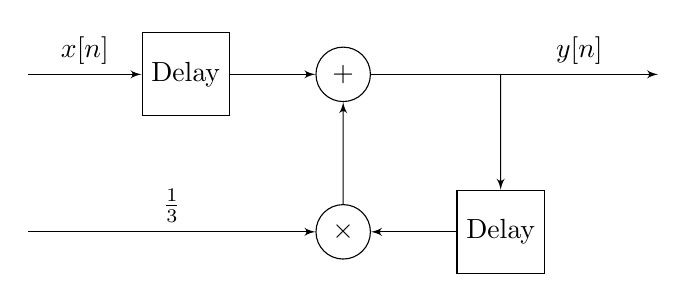
\begin{tikzpicture}[auto, node distance=2cm,>=latex']

                \node [input, name=input] {};
                \node [block, right of=input] (delay1) {Delay};
                \node [sum, right of=delay1, node distance=2cm] (sum) {$+$};
                \node [input, below of=delay1] (inv2) {};
                \node [input, below of=input] (constant) {};
                \node [sum, right of =constant, node distance = 4cm] (product) {$\times$};
                \node [input, right of=sum] (inv3) {};
                \node [block, right of=product] (delay2) {Delay};

                \node [output, right of=inv3] (output) {};
                \draw [draw,->] (input) -- node {$x[n]$} (delay1);
                \draw [draw,->] (delay1) -- (sum);
                \draw [draw,->] (constant) -- node{$\frac{1}{3}$} (product);
                \draw [draw,->] (product) --  (sum);
                \draw [draw,->] (delay2) --  (product);
                \draw [-] (sum) -- (inv3);
                \draw [->] (inv3) -- (delay2);
                \draw [->] (inv3) -- node [name=y] {$y[n]$}(output);
            \end{tikzpicture}
    \end{enumerate}
    \subsection{} Draw a block diagram representation for the following systems
    \begin{enumerate}
        \item[(a)] $y(t) = -\frac{1}{2}\frac{dy(t)}{dt}+4x(t)$ \\
            \begin{tikzpicture}[auto, node distance=2cm,>=latex']

                \node [input, name=input] {};
                \node [input, below of=input] (constant1) {$\frac{1}{2}$};
                \node [input, below of=constant1] (constant2) {$\frac{1}{2}$};
                \node [sum, right of=input] (product1) {$\times$};
                \node [sum, right of=product1] (sum) {$+$};
                \node [input, below of=product1] (inv1) {};
                \node [input, below of=inv1] (inv2) {};
                \node [sum, right of=inv2] (product2) {$\times$};
                \node [input, below of=sum] (constant3) {$\frac{1}{3}$};
                \node [input, right of=sum] (inv3) {};
                \node [block, right of=product2] (delay) {$\frac{d}{dt}$};
                \node [output, right of=inv3] (output) {};
                \draw [draw,->] (input) -- node {$x(t)$} (product1);
                \draw [draw,->] (product1) --  (sum);
                \draw [draw,-] (constant1) -- node {$4$} (inv1);
                \draw [draw,->] (inv1) --  (product1);
                \draw [draw,-] (constant2) -- node {$-\frac{1}{2}$} (inv2);
                \draw [draw,->] (inv2) --  (product2);
                \draw [draw,->] (product2) --  (sum);
                \draw [draw,->] (delay) --  (product2);
                \draw [-] (sum) -- (inv3);
                \draw [->] (inv3) -- (delay);
                \draw [->] (inv3) -- node [name=y] {$y[n]$}(output);
            \end{tikzpicture}
        \item[(b)] $y(t) = \frac{1}{3}[x(t)-\frac{dy(t)}{dt}]$ \\
    \end{enumerate}
\end{document}